\documentclass[pdf]{beamer}
\usepackage{listings}
\newcommand{\coqatoo}{Coqatoo}


\definecolor{grey}{rgb}{0.8,0.8,0.8}
\definecolor{code-background}{RGB}{255, 248, 220}
\definecolor{code-comment}{RGB}{196, 42, 42}
\definecolor{code-linenumber}{rgb}{0.5,0.5,0.5}
\definecolor{code-keyword}{RGB}{148, 0, 211}
\lstset{
   backgroundcolor=\color{code-background},   	% choose the background color; you must add \usepackage{color} or \usepackage{xcolor}
   basicstyle=\tt\small,       			% the size of the fonts that are used for the code
   breakatwhitespace=false,         			% sets if automatic breaks should only happen at whitespace
   breaklines=true,                 			% sets automatic line breaking
   captionpos=none,                    			% sets the caption-position to bottom
   commentstyle=\color{code-comment},   		% comment style
   deletekeywords={...},            			% if you want to delete keywords from the given language
   escapeinside={\%*}{*)},          			% if you want to add LaTeX within your code
   extendedchars=true,              			% lets you use non-ASCII characters; for 8-bits encodings only, does not work with UTF-8
   frame=tb,
   framerule=0pt,
   framextopmargin=0pt,
   framexbottommargin=0pt,
   keepspaces=true,                 			% keeps spaces in text, useful for keeping indentation of code (possibly needs columns=flexible)
   keywordstyle=\color{code-keyword},       						% keyword style
   language=ML,                 				% the language of the code
   morekeywords={Lemma, Proof, Qed},            % if you want to add more keywords to the set
   numbers=none,                    			% where to put the line-numbers; possible values are (none, left, right)
   numbersep=5pt,	                   			% how far the line-numbers are from the code
   numberstyle=\tiny\color{code-linenumber}, 	% the style that is used for the line-numbers
   rulecolor=\color{black}, 	        		% if not set, the frame-color may be changed on line-breaks within not-black text (e.g. comments (green here))
   showspaces=false,            	    		% show spaces everywhere adding particular underscores; it overrides 'showstringspaces'
   showstringspaces=false,          			% underline spaces within strings only
   showtabs=false,                  			% show tabs within strings adding particular underscores
   stepnumber=1,                    			% the step between two line-numbers. If it's 1, each line will be numbered
   stringstyle=\color{black},            		% string literal style
   tabsize=2,                       			% sets default tabsize to 2 spaces
   gobble=0,									% number of characters to remove at the beginning of each line
   mathescape=true,								% to render math symbols in the listing (between $)
   title=\lstname,                   			% show the filename of files included with \lstinputlisting; also try caption instead of title
   belowcaptionskip = 0cm
}
\usetheme{Luebeck} %default, AnnArbor, Antibes, Bergen, Berkeley, Berlin, Boadilla, CambridgeUS, Copenhagen, Darmstadt, Dresden, EastLansing, Frankfurt, Goettingen, Hannover, Ilmenau, JuanLesPins, Luebeck, Madrid, Malmoe, Marburg, Montpellier, PaloAlto, Pittsburgh, Rochester, Singapore, Szeged, Warsaw

\usecolortheme{beaver} %default, albatross, beaver, beetle, crane, dolphin, dove, fly, lily, orchid, rose, seagull, seahorse, whale, wolverine
%\useinnertheme{circle} %circles, rectangles, rounded, inmargin 
%\useoutertheme{tree} %infolines, smoothbars, sidebar, split, tree 

\definecolor{coqatoo-pink}      {RGB}{255, 107, 104}
\definecolor{coqatoo-gray}      {RGB}{64, 64, 64}
\definecolor{coqatoo-yellow}    {RGB}{239, 223, 0}

\setbeamercolor{palette primary}   {bg=coqatoo-pink,fg=white}
%\setbeamercolor{palette secondary} {bg=white,fg=black}
%\setbeamercolor{palette tertiary}  {bg=blue,fg=red}
%\setbeamercolor{palette quaternary}{bg=white,fg=black}
\setbeamercolor{structure}{fg=coqatoo-gray}
\setbeamercolor{titlelike}         {bg=coqatoo-pink,fg=white}
\setbeamercolor{frametitle}        {bg=coqatoo-pink,fg=white}
\setbeamercolor{normal text}       {bg=white,fg=coqatoo-gray}

\title[Coqatoo]{
\includegraphics[width=50pt]{images/logo.png}\\Coqatoo}
\subtitle{Generating Natural Language Versions of Coq Proofs}
\author{Andrew Bedford}
\institute{Laval University}
\date{CoqPL 2018}

\begin{document}

\begin{frame}
    \titlepage
\end{frame}

\begin{frame}{Motivation}
    \begin{itemize}
        \item Proofs can sometimes be hard to understand, particularly for less-experienced users
        \item CtCoq and its successor Pcoq are no longer available
    \end{itemize}
\end{frame}

\begin{frame}[fragile]{Example}{Input}
    \begin{lstlisting}[label=listing:input]
    Lemma conj_imp_equiv : forall P Q R:Prop, 
        (P /\ Q -> R) <-> (P -> Q -> R).
    Proof.
        intros. split. intros H HP HQ. apply H. apply conj. assumption. assumption. intros H HPQ. inversion HPQ. apply H. assumption. assumption.
    Qed.
    \end{lstlisting}
\end{frame}

\begin{frame}
    Coqatoo’s rewriting algorithm can be decomposed in three steps:
    \begin{enumerate}
        \item Information extraction
        \item Proof tree construction
        \item Tactic-based rewriting
    \end{enumerate}
\end{frame}


\begin{frame}[fragile]{Step 1: Information extraction}
    Coqatoo captures the intermediary proof states
    \begin{lstlisting}[label=listing:before-intros, captionpos=b,caption={State before executing the first intros tactic}]
    1 subgoal

    ============================
    forall P Q R : Prop, (P /\ Q -> R) <-> (P -> Q -> R)
    \end{lstlisting}

    \begin{lstlisting}[label=listing:after-intros,captionpos=b,caption={State after executing the first intros tactic}]
    1 subgoal

    P, Q, R : Prop
    ============================
    (P /\ Q -> R) <-> (P -> Q -> R)
    \end{lstlisting}
\end{frame}

\begin{frame}{Step 2: Proof tree construction}
    \vspace{-13pt}\center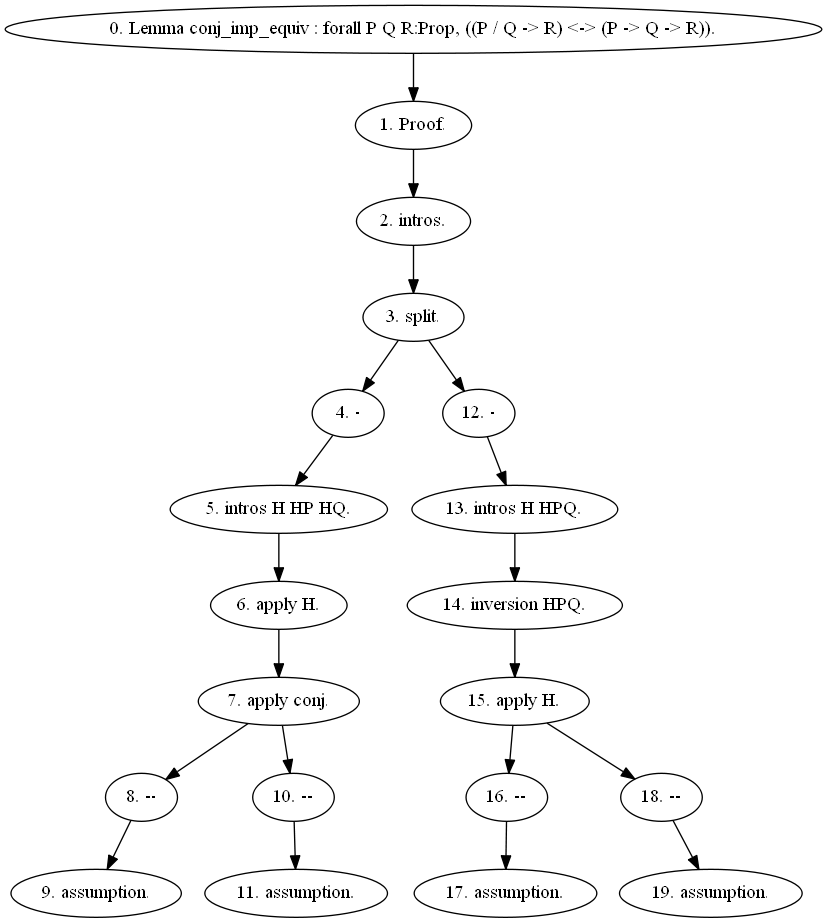
\includegraphics[height=0.85\textheight]{images/proof-tree.png}
\end{frame}

\begin{frame}{Step 3: Tactic-based rewriting}

\end{frame}

\begin{frame}[fragile]{Example}{Output}
\begin{lstlisting}[label=listing:output, captionpos=b, caption={Output in annotation mode},basicstyle=\tt\tiny]
Lemma conj_imp_equiv : forall P Q R:Prop, ((P /\ Q -> R) <-> (P -> Q -> R)).
Proof.
  (* Assume that P, Q and R are arbitrary objects of type Prop. Let us show that (P /\ Q -> R) <-> (P -> Q -> R) is true. *) intros.
  split.
  - (* Case (P /\ Q -> R) -> P -> Q -> R: *) 
    (* Suppose that P, Q and P /\ Q -> R are true. Let us show that R is true. *) intros H HP HQ.
    (* By our hypothesis P /\ Q -> R, we know that R is true if P /\ Q  is true. *) apply H.
    apply conj.
    -- (* Case P: *)
       (* True, because it is one of our assumptions. *) assumption.
    -- (* Case Q: *)
       (* True, because it is one of our assumptions. *) assumption.
  - (* Case (P -> Q -> R) -> P /\ Q -> R: *)
    (* Suppose that P /\ Q and P -> Q -> R are true. Let us show that R is true. *) intros H HPQ.
    (* By inversion on P /\ Q, we know that P, Q are also true. *) inversion HPQ.
    (* By our hypothesis P -> Q -> R, we know that R is true if P and Q are true. *) apply H.
    -- (* Case P: *)
       (* True, because it is one of our assumptions. *) assumption.
    -- (* Case Q: *)
       (* True, because it is one of our assumptions. *) assumption.
Qed.
\end{lstlisting}
\end{frame}

\begin{frame}
    \Huge \center Demonstration
\end{frame}

\begin{frame}{Comparison}{Disadvantages}
    \begin{itemize}
        \item{It only works on proofs whose tactics are supported, while the approach of Coscoy et al. worked on any proof.}
        \item{It may require additional verifications to ensure that unecessary information (e.g., an assertion which isn't used) is not included in the generated proof.}
    \end{itemize}
\end{frame}

\begin{frame}{Comparison}{Advantages}
    \begin{itemize}
        \item{It enables us to more easily control the size and verbosity of the generated proof (one or two sentences per tactic by default).}
        \item{It maintains the order and structure of the user's original proof script; this is not necessarily the case in Coscoy et al. }
      \end{itemize}
\end{frame}

\begin{frame}{Future work}
    \begin{itemize}
        \item Increase the number of supported tactics
        \begin{itemize}
            \item Goal: Software Foundations
        \end{itemize}
        \item Add partial support for automation
        \item Integration with existing development environments
        \item Add a LaTeX output mode
    \end{itemize}
\end{frame}

\end{document}